\documentclass{beamer}

\usepackage[frenchb]{babel}
\usepackage[T1]{fontenc}
\usepackage[utf8]{inputenc}

\usetheme{Warsaw}
\useoutertheme{infolines}

\usepackage{amsmath}
\usepackage{amssymb}
\usepackage{amsthm}
\usepackage{stmaryrd}

\usepackage[all]{xy}

\setbeamercovered{transparent}

\begin{document}

\title{Monades, Comonades et Automates cellulaires}
\author{Jérémy S. Cochoy}
\institute{INRIA Paris-Saclay}
\date{Octobre 2015}


\begin{frame}
\titlepage
\end{frame}

\begin{frame}
  \begin{columns}[t]
  \begin{column}{5cm}
  \tableofcontents[sections={1-3}]
  \end{column}
  \begin{column}{5cm}
  \tableofcontents[sections={4-8}]
  \end{column}
  \end{columns}
\end{frame}

\begin{frame}

\begin{center}

\includegraphics[scale=0.3]{screen1.png}
\end{center}

\end{frame}

\section{Monades}

\subsection{Types}
\begin{frame}
\frametitle{Les types}
\begin{block}{Qu'est-ce qu'un type?}
C'est un \emph{ensemble} de valeurs.
\end{block}
\pause
\begin{exampleblock}{Exemples :}
\begin{itemize}
\item $Int = \{-2 147 483 648, \dots, 2 147 483 647\}$
\item $Bool = \{True, False\}$
\item $Char = \{'a', 'b', 'c' , \dots\}$
\pause
\item $[Bool] = \{[], [True], [False], [True, False], [False, True], \dots\}$
\pause
\item $[a]$
\end{itemize}

\end{exampleblock}
\end{frame}

\begin{frame}
\frametitle{Les types}
\begin{block}{Construire son type :}
\begin{itemize}
\item Trival = Plus | Minus | Zero
\pause
\item Box a = InABox a
\pause
\item Maybe a = Just a | Nothing
\pause
\item Either a b = Left a | Right b
\end{itemize}
\end{block}

\pause

Just, Nothing, InABox etc portent le doux nom de \emph{constructeur de type}. C'est aussi le cas de \emph{[]}.
\end{frame}

\subsection{Fonctions}
\begin{frame}
\frametitle{Les fonctions}
\begin{block}{}
Ce sont les traitements que l'on peut implémenter.
\end{block}
\begin{center}

\includegraphics[scale=0.2]{fct.png}
\end{center}
\pause
\begin{block}{}
Une fonction ne lance pas de missile.
\end{block}
\end{frame}


\begin{frame}
\frametitle{Les fonctions}
\begin{block}{Une fonction a aussi un type : \emph{a -> b}}
\begin{itemize}
\item floor   :: Float -> Int
\item (+2):: Int -> Int
\pause
\item id      :: a -> a
\item map :: (a -> b) -> [a] -> [b]
\end{itemize}
\end{block}

\end{frame}


\begin{frame}
\frametitle{Les fonctions}
\begin{block}{Ça se compose}
\begin{itemize}
\item f1 :: a -> b
\item f2 :: b -> c
\item f2 . f1 :: a -> c
\pause
\item . :: (a -> b) -> (b -> c) -> (a -> c)
\end{itemize}
\end{block}
\pause

La collection de tous les types forme une catégorie. Les flèches sont les fonctions implémentables. On l’appelle la catégorie des types.

\end{frame}

\subsection{Foncteurs}


\begin{frame}
\frametitle{Les foncteurs}
\begin{block}{Un foncteur F agit sur les types ...}
\begin{itemize}
\item a => F a
\end{itemize}
\end{block}
\begin{exampleblock}{}
\begin{itemize}
\item a => Maybe a
\item a => [a]
\end{itemize}
\end{exampleblock}

\pause

\begin{block}{... et sur les fonctions}
\begin{itemize}
\item a -> b => F a -> F b
\end{itemize}
\end{block}

\begin{exampleblock}{}
\begin{itemize}
\item fmap (+2) :: F Int -> F Int
\item fmap id :: F a -> F a
\end{itemize}
\end{exampleblock}
\end{frame}

\begin{frame}
\frametitle{Donnée dans un contexte}

\begin{center}
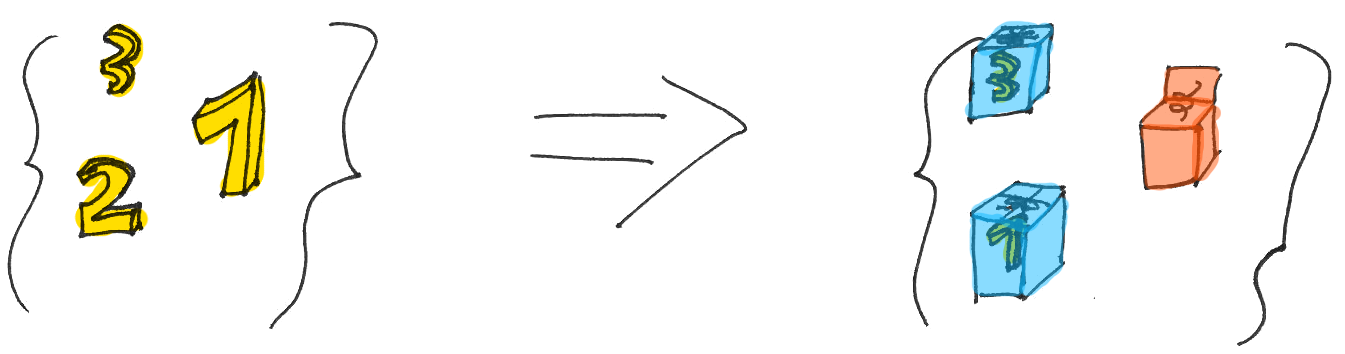
\includegraphics[scale=0.25]{a2fa.png}
\end{center}

\begin{block}{}
Un foncteur permet de passer d'un monde (les types a) vers un autre (les types F a).
\end{block}

\end{frame}

\begin{frame}
\frametitle{Functorial mapping}
On ne peut plus appliquer la fonction telle qu'elle les diagrammes suivant commutent :

\begin{center}
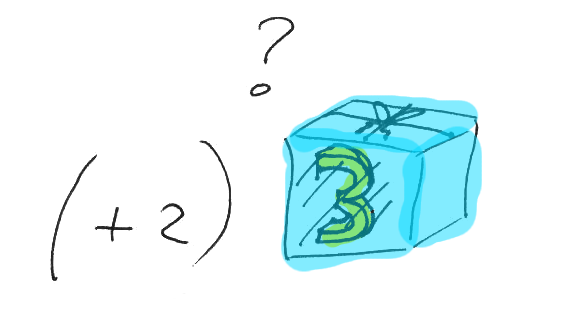
\includegraphics[scale=0.3]{wrong_type.png}
\end{center}
\end{frame}

\begin{frame}
\frametitle{Functorial mapping}
Mais le foncteur nous donne une nouvelle flèche.
\begin{center}
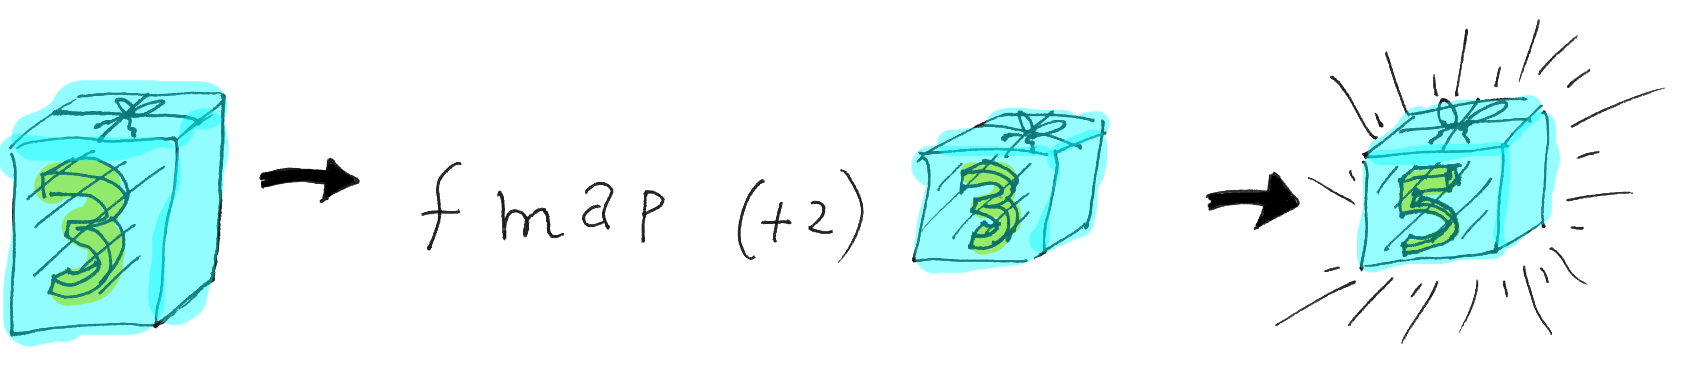
\includegraphics[scale=0.19]{f_fct.png}
\end{center}
\end{frame}



\begin{frame}
\frametitle{Dura lex sed lex}
\begin{alertblock}{Un foncteur doit respecter des lois}
\begin{itemize}
\item fmap id = id
\item fmap (p . q) = (fmap p) . (fmap q)

\end{itemize}
\end{alertblock}

\pause
Un foncteur est un endofoncteur de la catégorie des types.
\end{frame}

\subsection{Monades}

\begin{frame}

\frametitle{Monades}
\begin{center}
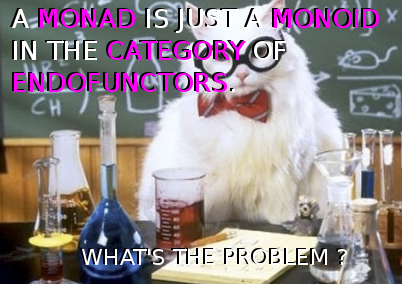
\includegraphics[scale=0.7]{cat.png}
\end{center}
\end{frame}

\begin{frame}
\frametitle{Donnée dans un contexte}

\begin{block}{}
Une monade place une valeur dans un contexte.
\end{block}

\begin{center}
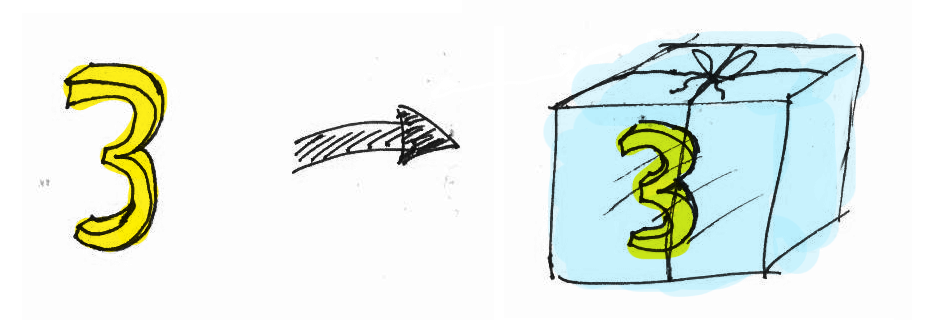
\includegraphics[scale=0.3]{just3.png}
\end{center}

\begin{exampleblock}{}
L'exemple de Maybe : \verb!Just 3!
\end{exampleblock}
\end{frame}

\begin{frame}
\frametitle{Donnée dans un contexte}

\begin{block}{}
Un contexte peut aussi ne pas contenir de valeur.
\end{block}

\begin{center}
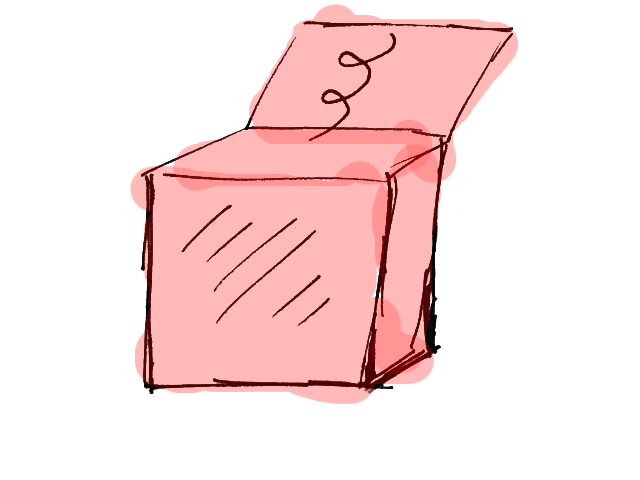
\includegraphics[scale=0.3]{nothing.png}
\end{center}
\begin{exampleblock}{}
L'exemple de Maybe : \verb!Nothing!
\end{exampleblock}
\end{frame}

\begin{frame}
\frametitle{Placer une donnée dans un contexte}

\begin{block}{L'opérateur \emph{pure}}
\begin{center}
\verb!pure :: a -> F a!
\end{center}
\end{block}

\begin{exampleblock}{Quelques cas particuliers}
	\begin{itemize}
		\item Just
		\item (: [])
		\item Right
	\end{itemize}
\end{exampleblock}
\end{frame}


\begin{frame}
\frametitle{Un traitement qui peut échouer}

\begin{center}
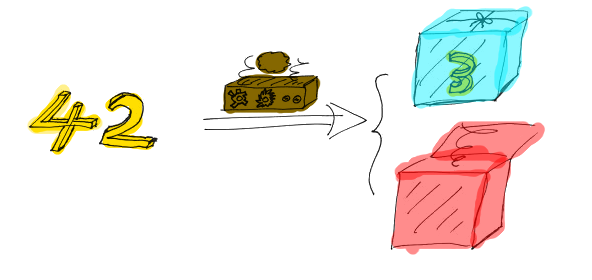
\includegraphics[scale=0.5]{failure.png}
\end{center}
\begin{exampleblock}{}
Une fonction de type \emph{Int -> Maybe Int}.
\end{exampleblock}
\end{frame}

\begin{frame}
\frametitle{Composer des traitements avec échec}
\begin{block}{}
Comment composer \verb!f :: a -> M b! et \verb!g :: b -> M c! ?
\end{block}
\pause
\begin{block}{}
Si $M$ est un foncteur, on peut composer
\verb!f :: a -> M b! avec \verb!fmap g :: M b -> M (M c)!.
\end{block}
\pause
\begin{block}{}
Que faire d'un \verb!M (M c)!?
\end{block}

\end{frame}

\begin{frame}
\frametitle{L'opérateur join}
\begin{block}{}
\begin{center}
\verb!join :: M (M a) -> M a!
\end{center}
\end{block}

\begin{center}
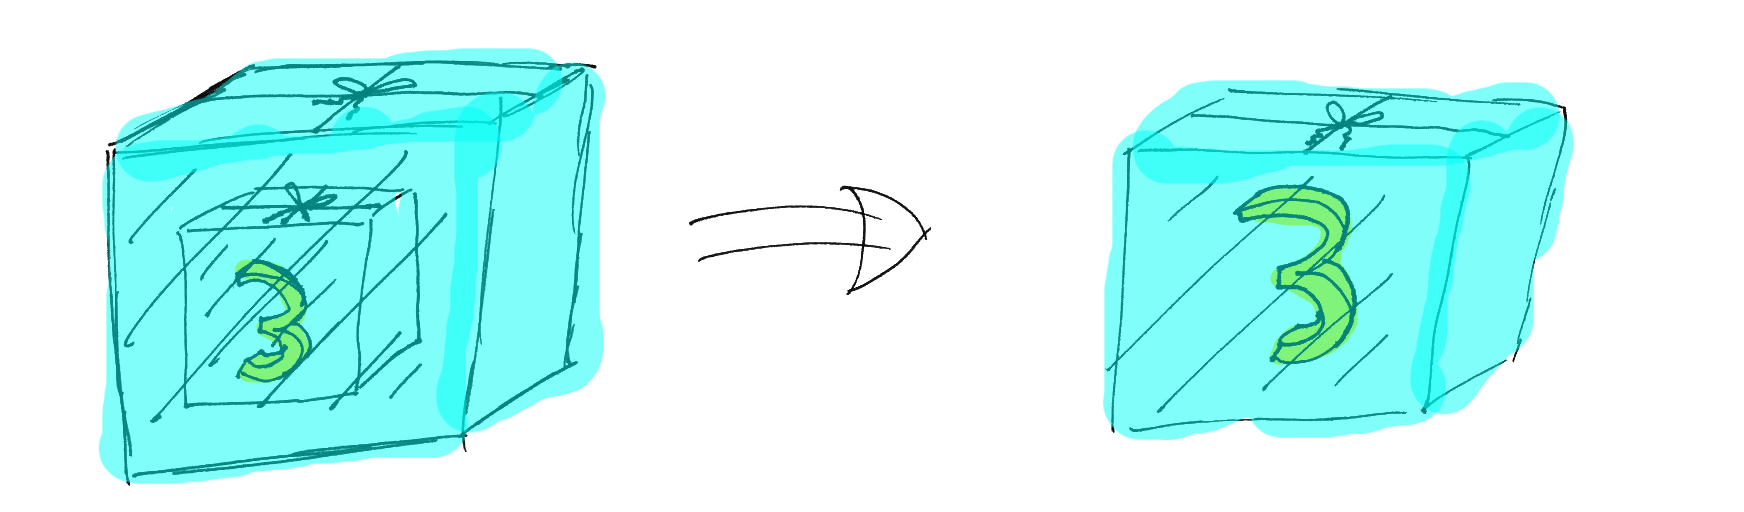
\includegraphics[scale=0.2]{join.png}
\end{center}
\pause
\begin{exampleblock}{}
\begin{center}
\verb!join \$ Just (Just 3)!.
\end{center}
\end{exampleblock}
\end{frame}


\begin{frame}
\frametitle{L'opérateur join}
\begin{block}{}
\begin{center}
\verb!join :: M (M a) -> M a!
\end{center}
\end{block}
\medskip
\begin{center}
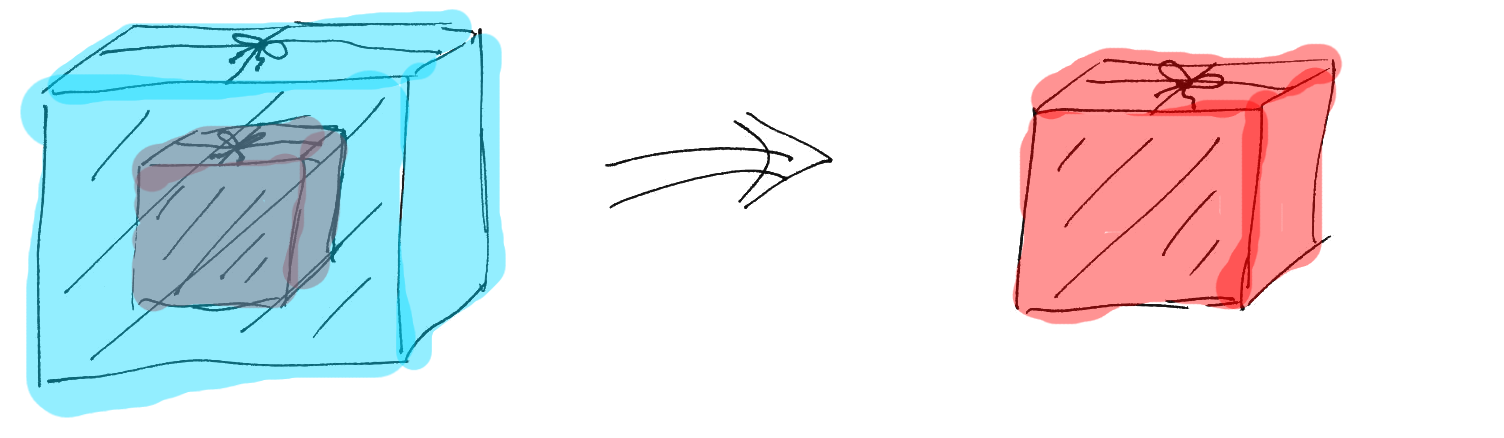
\includegraphics[scale=0.2]{join_nothing.png}
\end{center}
\medskip
\pause
\begin{exampleblock}{}
\begin{center}
\verb!join \$ Just (Nothing)!.
\end{center}
\end{exampleblock}
\end{frame}



\begin{frame}
\frametitle{L'opérateur \emph{bind}}
\begin{block}{On cherche à définir la composition.}
\verb!(>=>) :: (a -> M b) -> (b -> M c) -> (a -> M c)!
\end{block}

\pause

\begin{block}{Nous avons :}
\begin{itemize}
\item \verb!(fmap g) . f :: a -> M (M c)!
\item \verb!join :: M (M a) -> M a!
\end{itemize}
\end{block}
\pause

\begin{block}{On peut maintenant composer $f$ et $g$.}

\verb!f >=> g $\equiv$ join . (fmap g) . f!.
\end{block}
\end{frame}

\begin{frame}
\frametitle{Récapitulatif}

\begin{block}{Une monade, c'est}

	\begin{itemize}
		\item fmap :: (a -> b) -> (M a -> M b)
		\item pure :: a -> M a
		\item join :: M (M a) -> M a
	\end{itemize}

\end{block}

\end{frame}

\begin{frame}
\frametitle{Dura lex sed lex}
\begin{alertblock}{Une monade doit respecter des lois}
\begin{itemize}
\item \verb!pure . f $\equiv$ (fmap f) . pure!
\item \verb!join . fmap (fmap f) $\equiv$ (fmap f) . join!
\item[] \ 
\item \verb!join . fmap join   $\equiv$ join . join!
\item \verb!join . fmap pure   $\equiv$ join . pure = id!
\end{itemize}
\end{alertblock}
\end{frame}

\begin{frame}
\frametitle{Monades - Catégories}
Une monade $(T, \mu, \eta)$ est la donnée d'un
endofoncteur $T : C \rightarrow C$ et de deux
transformations naturelles $\mu : T\circ T \rightarrow T$ et $\eta : 1_C \rightarrow T$ telles que :

\[
\begin{array}{cc}
\xymatrix{
T(T(T(X))) \ar[r]^{T(\mu_X)} \ar[d]_{\mu_{T(X)}} & T(T(X)) \ar[d]^{\mu_X} \\
T(T(X)) \ar[r]_{\mu_X} & T(X) \\
}
&
\xymatrix{
T(X) \ar[r]^{\eta_{T(X)}} \ar[d]_{T(\eta_X)}  \ar@{=}[dr] & T(T(X)) \ar[d]^{\mu_X} \\
T(T(X)) \ar[r]_{\mu_X} & T(X) \\
}
\end{array}
\]
c'est à dire
$\mu \circ T\mu = \mu \circ \mu_T$
et
$\mu \circ T \eta = \mu \circ \eta_T = id_T$.

\pause

Dans notre cas, $C$ est la catégorie des types.
\end{frame}

\begin{frame}
\frametitle{A chaque loi son diagramme}
\begin{alertblock}{\verb!pure! est une T.N.}
\verb!pure . f $\equiv$ (fmap f) . pure!
\end{alertblock}

\begin{block}{}
\[
\xymatrix{
X \ar[r]^{f} \ar[d]_{\eta_X} & Y \ar[d]^{\eta_Y} \\
T(X) \ar[r]_{T(f)} & T(Y) \\
}
\]
\end{block}

\end{frame}

\begin{frame}
\frametitle{A chaque loi son diagramme}
\begin{alertblock}{\verb!join! est une T.N.}
\verb!join . fmap (fmap f) $\equiv$ (fmap f) . join!
\end{alertblock}

\begin{block}{}
\[
\xymatrix{
T(T(X)) \ar[r]^{T(T(f))} \ar[d]_{\mu_{X}} & T(T(Y)) \ar[d]^{\mu_{Y}} \\
T(X) \ar[r]_{T(f)} & T(Y) \\
}
\]
\end{block}

\end{frame}


\begin{frame}
\frametitle{A chaque loi son diagramme}
\begin{alertblock}{Associativité}
\verb!join . fmap join   $\equiv$ join . join!
\end{alertblock}

\begin{block}{}

\[
\xymatrix{
T(T(T(X))) \ar[r]^{T(\mu_X)} \ar[d]_{\mu_{T(X)}} & T(T(X)) \ar[d]^{\mu_X} \\
T(T(X)) \ar[r]_{\mu_X} & T(X) \\
}
\]
\end{block}

\begin{block}{}
\begin{center}
$\mu \circ T\mu = \mu \circ \mu_T$
\end{center}
\end{block}

\end{frame}

\begin{frame}
\frametitle{A chaque loi son diagramme}
\begin{alertblock}{Existence d'un neutre}
\verb!join . fmap pure   $\equiv$ join . pure = id!
\end{alertblock}

\begin{block}{}
\[
\xymatrix{
T(X) \ar[r]^{\eta_{T(X)}} \ar[d]_{T(\eta_X)}  \ar@{=}[dr] & T(T(X)) \ar[d]^{\mu_X} \\
T(T(X)) \ar[r]_{\mu_X} & T(X) \\
}
\]
\end{block}

\begin{block}{}
\begin{center}
$\mu \circ T \eta = \mu \circ \eta_T = id_T$
\end{center}
\end{block}

\end{frame}


\section{Automates Cellulaires}

\subsection{Qu'est-ce que c'est?}

\begin{frame}
\begin{center}
\textbf{Automates cellulaires}
\end{center}

\begin{center}
%
\includegraphics[scale=0.5]{automata_flip.png}
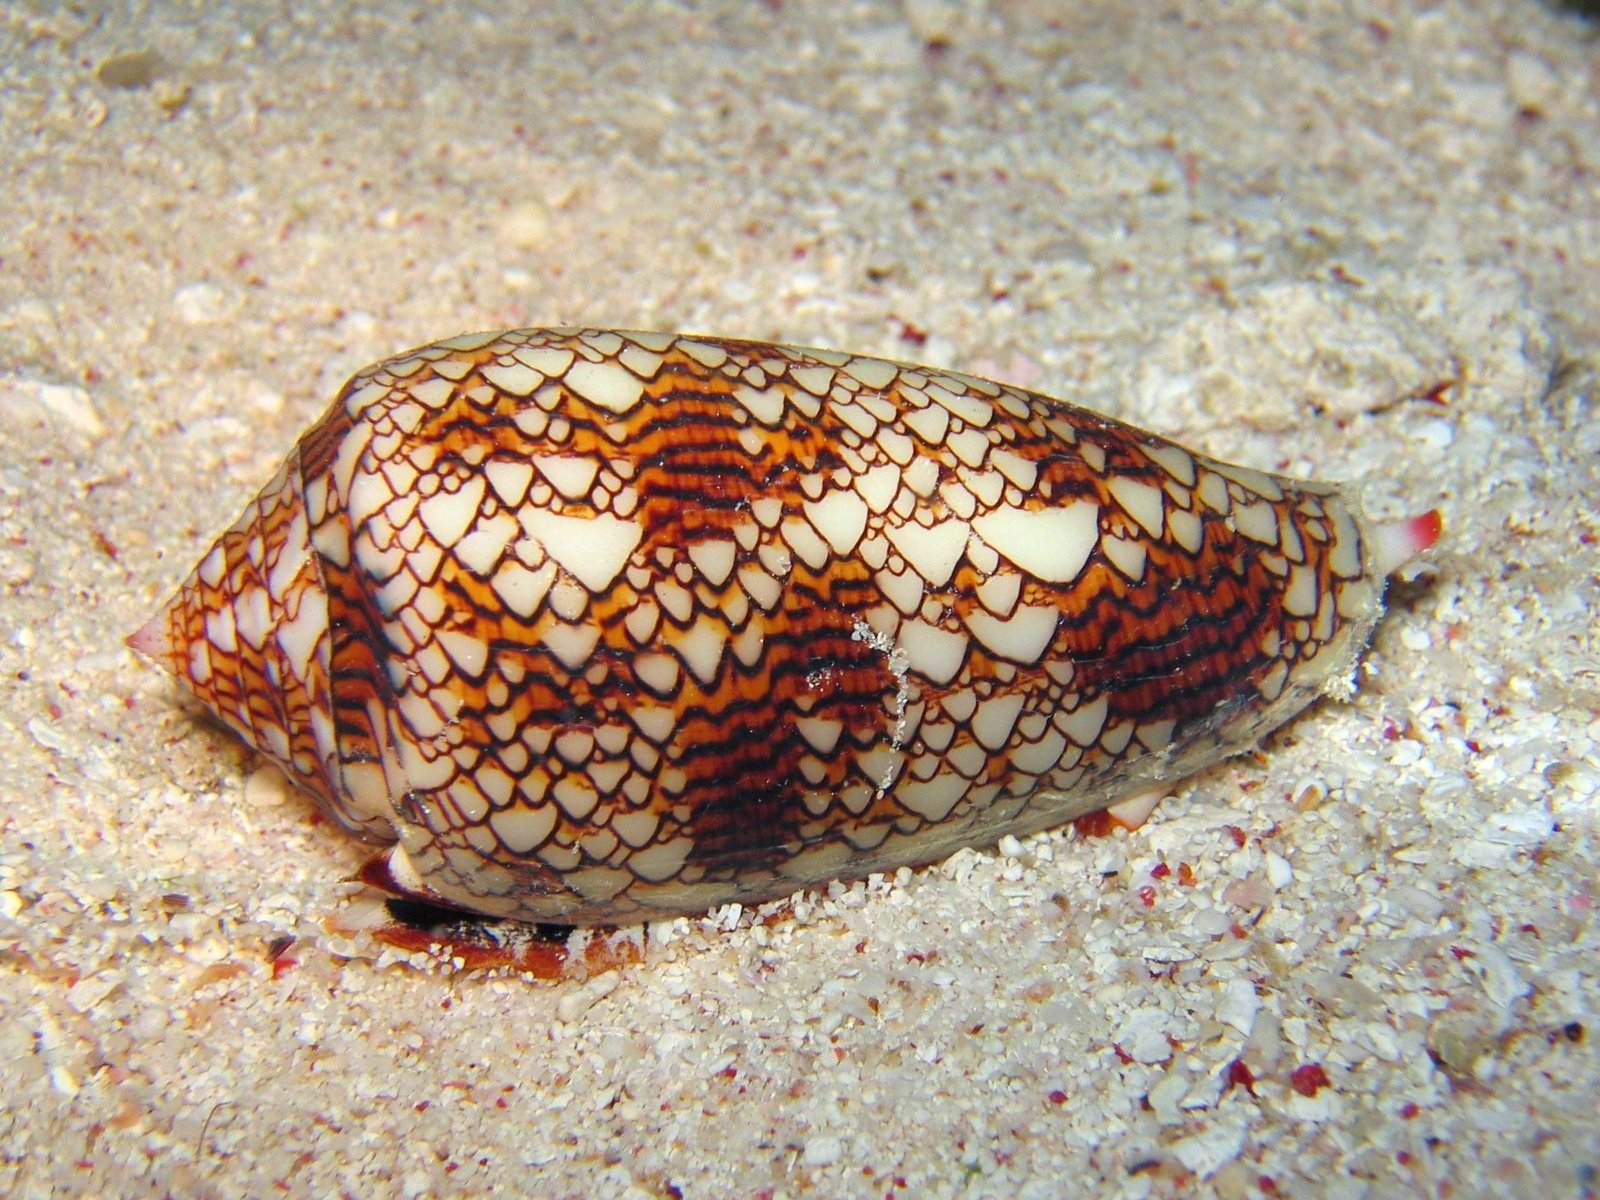
\includegraphics[scale=0.16]{textile_cone.jpg}
\end{center}

\begin{center}Toison d'or\end{center}

\end{frame}


\begin{frame}
\frametitle{Qu'est-ce qu'un automate cellulaire?}
\begin{block}{Un automate cellulaire, c'est :}
	\begin{itemize}
		\item Un nombre fini d'états $S$,
		\item Une grille de cellules,
		\item La notion de voisinage d'une cellule $V_c$,
		\item Une fonction de transition qui à une cellule associe son nouvel état.
	\end{itemize}
\end{block}
\end{frame}

\begin{frame}
\frametitle{Combien d'automates cellulaires différents?}
\begin{block}{On a le choix :}
	\begin{itemize}
	\item De la dimension de la grille,
	\item Des lois,
	\item Du nombres d'états (couleurs),
	\item De la forme du voisinages (boules de rayon r, etc.),
	\item De ne pas être déterministe.
	\end{itemize}
\end{block}
\end{frame}

\subsection{Le jeu de la vie}
\begin{frame}
\frametitle{The "Game of Life"}
\begin{center}
\bf{Jeu de la vie} (J. H. Conway)
\end{center}
\begin{center}
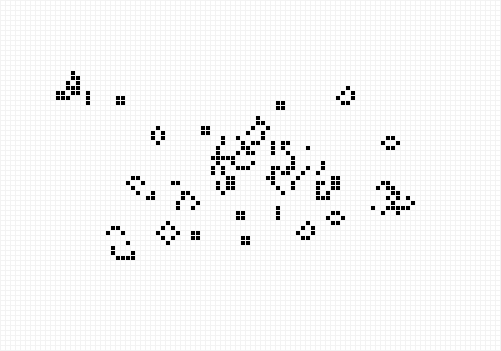
\includegraphics[scale=0.5]{game_of_life.png}
\end{center}
\end{frame}

\begin{frame}
\frametitle{Étude d'un cas : Rule 30}
\begin{center}
\textbf{Rule 30}
\end{center}
\begin{center}

\includegraphics[scale=1]{rule30.png}
\end{center}
\end{frame}

\subsection{Algorithme 1D}
\begin{frame}
\frametitle{La grille}
\begin{block}{La grille de l'automate}
\begin{center}

\includegraphics[scale=0.5]{grid.png}
\end{center}
\end{block}
\begin{itemize}
	\item Une grille 1D
	\item Deux états (Blanc / Noir)
\end{itemize}
\end{frame}

\begin{frame}
\begin{block}{}
	Un voisinage de 3 cellules.
\end{block}
\pause
\begin{block}{Les règles}
	\begin{center}
	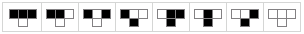
\includegraphics[scale=1]{rule30_rule.png}
	\end{center}
\end{block}
\pause
\begin{block}{On peut aussi écrire :}
	\begin{center}
	\begin{tabular}{|l|c|c|c|c|c|c|c|c|}
	\hline
	Ancien état & 111 & 110 & 101 & 100 & 011 & 010 & 001 & 000 \\
	\hline
	Nouvel état	& 0   & 0   & 0   & 1   & 1   & 1   & 1   & 0 \\
	\hline
	\end{tabular}
	\end{center}
\end{block}
\end{frame}

\section{Comonades}

\begin{frame}
\begin{center}
\textbf{Comonades}
\end{center}

\begin{center}
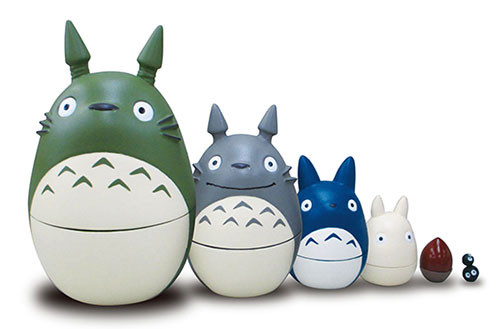
\includegraphics[scale=0.5]{comonad.jpg}
\end{center}
\end{frame}

\begin{frame}
\frametitle{C'est le dual d'une monade}

\begin{itemize}
\item C'est un foncteur M
\item extract (copure) (co uinit) :: M a -> a
\item duplicate (cojoin) (co product $\delta$) :: M a -> M (M a)
\end{itemize}
\end{frame}

\begin{frame}
\frametitle{Dura lex sed lex}
\begin{alertblock}{Une comonade doit respecter des lois}
\begin{itemize}
\item \verb!(fmap (fmap f)) . duplicate $\equiv$ duplicate . fmap f!
\item \verb!duplicate . duplicate = fmap duplicate . duplicate!
\item[] \ 
\item \verb!duplicate . duplicate $\equiv$ fmap duplicate . duplicate! (commut)
\item \verb!fmap extract . duplicate $\equiv$ extract . duplicate $\equiv$ id! (co unit)
\end{itemize}
\end{alertblock}
\end{frame}


\begin{frame}
\frametitle{Comonades - Catégories}
Une comonade $(T, \delta, \epsilon)$ est la donnée d'un
endofoncteur $T : C \rightarrow C$ et de deux
transformations naturelles $\Delta : T \rightarrow T\circ T$ et $\epsilon : T \rightarrow 1_C$ telles que :

\[
\begin{array}{cc}
\xymatrix{
T(X) \ar[r]^{\Delta_X} \ar[d]_{\Delta_X} & T(T(X)) \ar[d]^{\Delta_{T(X)}} \\
T(T(X)) \ar[r]_{T(\Delta_X)} & T(T(T(X))) \\
}
&
\xymatrix{
T(X) \ar[d]_{\Delta_X} \ar[r]^{\Delta_X}  \ar@{=}[dr] & T(T(X))   \ar[d]^{\epsilon_{T(X)}} \\
T(T(X)) \ar[r]_{T(\epsilon_X)} & T(X) \\
}
\end{array}
\]
c'est à dire
$\Delta_T \circ \Delta = T \Delta \circ \Delta$
et
$T \epsilon \circ \Delta = \epsilon_T \circ \Delta = id$.
\end{frame}

\begin{frame}
\frametitle{A chaque loi son diagramme}
\begin{alertblock}{\verb!extract! est une T.N.}
\verb!f . extract $\equiv$ extract . (fmap f)!
\end{alertblock}

\begin{block}{}
\[
\xymatrix{
X \ar[r]^{f} & Y  \\
T(X) \ar[r]_{T(f)} \ar[u]_{\epsilon_X} & T(Y) \ar[u]^{\epsilon_Y}\\
}
\]
\end{block}

\end{frame}

\begin{frame}
\frametitle{A chaque loi son diagramme}
\begin{alertblock}{\verb!duplicate! est une T.N.}
\verb!(fmap (fmap f)) . duplicate $\equiv$ duplicate . fmap f!
\end{alertblock}

\begin{block}{}
\[
\xymatrix{
T(X) \ar[r]_{T(f)} \ar[d]_{\Delta_{X}} & T(Y) \ar[d]^{\Delta_{Y}} \\
T(T(X)) \ar[r]^{T(T(f))} & T(T(Y)) \\
}
\]
\end{block}

\end{frame}


\begin{frame}
\frametitle{A chaque loi son diagramme}
\begin{alertblock}{Coassociativité}
\verb!duplicate . duplicate = fmap duplicate . duplicate!
\end{alertblock}

\begin{block}{}

\[
\xymatrix{
T(X) \ar[r]^{\Delta_X} \ar[d]_{\Delta_X} & T(T(X)) \ar[d]^{\Delta_{T(X)}} \\
T(T(X)) \ar[r]_{T(\Delta_X)} & T(T(T(X))) \\
}
\]
\end{block}

\begin{block}{}
\begin{center}
$\Delta_T \circ \Delta = T\Delta \circ \Delta$
\end{center}
\end{block}

\end{frame}

\begin{frame}
\frametitle{A chaque loi son diagramme}
\begin{alertblock}{Existence d'une counité}
\verb!extract . duplicate = fmap extract . duplicate = id!
\end{alertblock}

\begin{block}{}
\[
\xymatrix{
T(X) \ar[d]_{\Delta_X} \ar[r]^{\Delta_X}  \ar@{=}[dr] & T(T(X))   \ar[d]^{\epsilon_{T(X)}} \\
T(T(X)) \ar[r]_{T(\epsilon_X)} & T(X) \\
}
\]
\end{block}

\begin{block}{}
\begin{center}
$\epsilon_T \circ \Delta = T \epsilon \circ \Delta = id_T$
\end{center}
\end{block}

\end{frame}

\section{Évaluer un automate est comonadique}

\begin{frame}
\begin{center}
\textbf{ Evaluer un automate est comonadique }
\end{center}
\begin{center}

\includegraphics[scale=0.5]{automata_flip.png}
\end{center}
\end{frame}

\subsection{Un univers}
\begin{frame}
\frametitle{L'univers}
\begin{center}
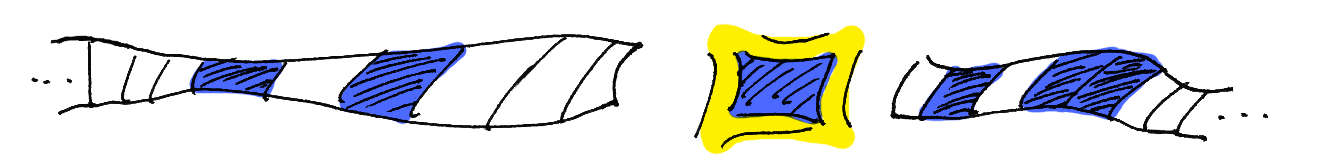
\includegraphics[scale=0.23]{ribbon_struct.png}
\end{center}

\begin{block}{Un ruban}
On représente l'univers dans lequel vie notre automate par un ruban, que l'on voit comme trois parties :

\begin{itemize}
\item La partie infinie à gauche
\item La case observée
\item La partie infinie à droite
\end{itemize}
\end{block}

\begin{block}{}
data Universe a = Universe [a] a [a]
\end{block}
\end{frame}

\begin{frame}
\frametitle{Quelques opérations sur notre univers}

\begin{center}

\includegraphics[scale=0.25]{ribbon_left.png}
\end{center}
\begin{block}{Voyageons}
On s'autorise à effectuer quelques opérations raisonnables sur notre univers :
\begin{itemize}
\item Regarder à gauche (left shift)
\item Regarder à droite (right shift)
\end{itemize}
\end{block}
\pause
\begin{block}{}
Moralement, on \emph{translate} notre ruban.
\end{block}
\pause
\begin{block}{}
left, right :: Universe a -> Universe a
\end{block}
\end{frame}

\subsection{Un foncteur}
\begin{frame}
\frametitle{L'univers est fonctoriel}
\begin{block}{Un foncteur}
Notre ruban est naturellement un foncteur : il suffit d'appliquer à notre \verb!Universe a! une fonction \verb!a -> b! sur chacune des cellules pour obtenir un \verb!Universe b!.
\end{block}
\begin{block}{}
fmap :: (a -> b) -> Universe a -> Universe b
\end{block}
\end{frame}

\subsection{Une comonade}
\begin{frame}
\frametitle{Comonades, nous voilà : extract}

\begin{center}
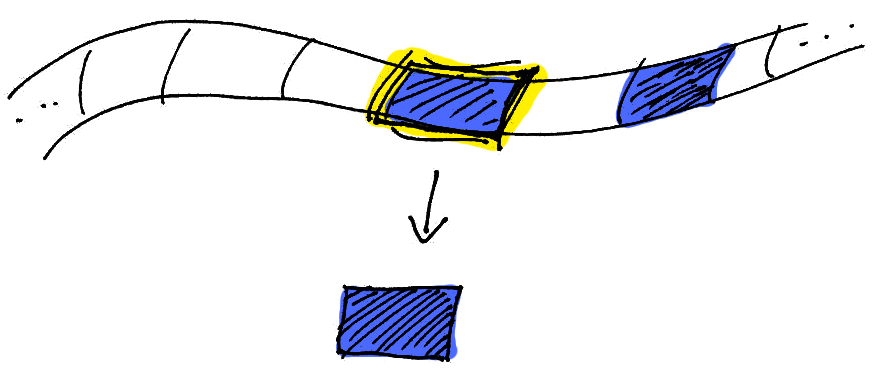
\includegraphics[scale=0.3]{ribbon_extract.png}
\end{center}
\begin{block}{Extraire une information}
Depuis notre univers, on peut extraire une valeur : celle de la case que l'on est en train d'observer!

\end{block}
\begin{block}{}
extract :: Universe a -> a
\end{block}
\end{frame}

\begin{frame}
\frametitle{Comonades, nous voilà : duplicate}
\begin{center}
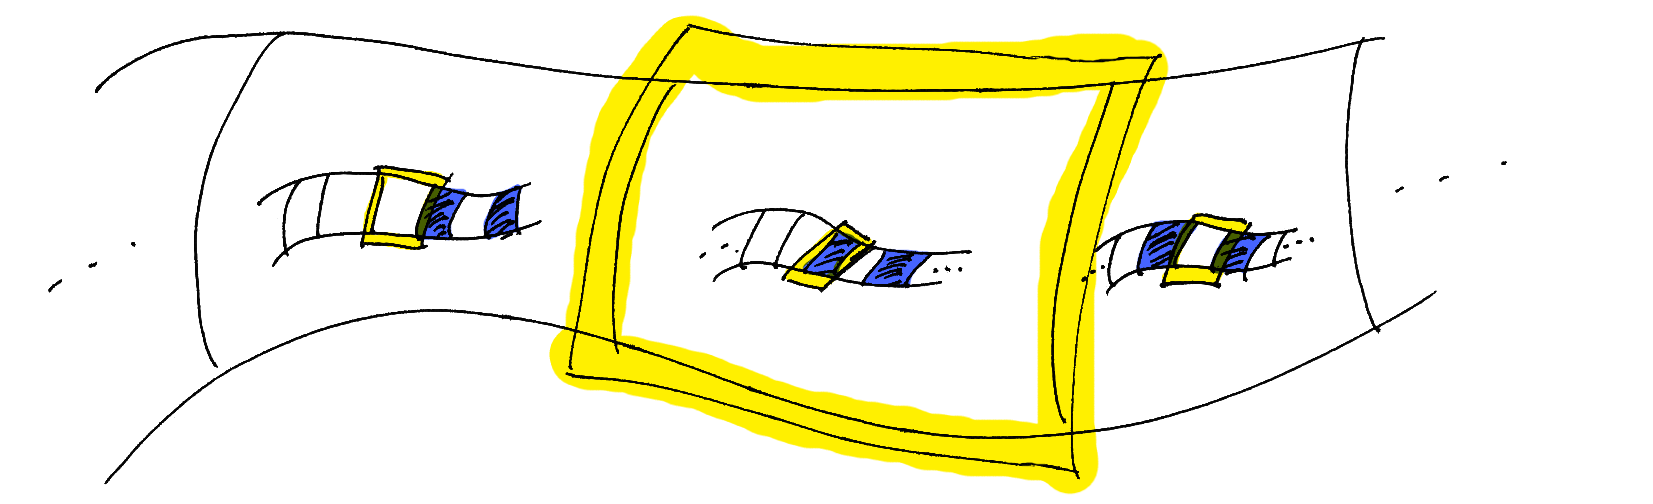
\includegraphics[scale=0.15]{ribbon_duplicate.png}
\end{center}

\begin{block}{L'opération duplicate}
On veut construire un univers où chaque case du ruban contient elle-même... un univers. Il s'agit de contenir tous les shift possible de notre univers de départ.
\end{block}

\begin{block}{}
duplicate :: Universe a -> Universe (Universe a)
\end{block}
\end{frame}

\subsection{Evaluation}

\begin{frame}
\frametitle{Loi de convolution}
\begin{center}
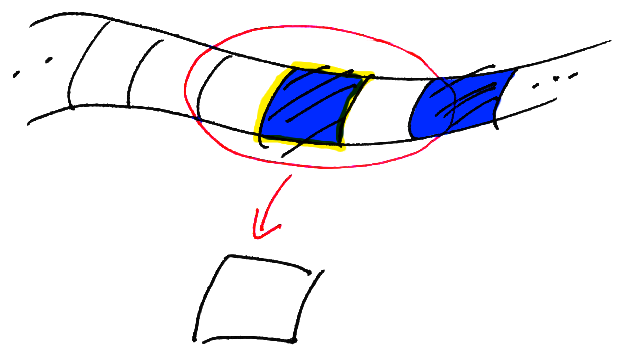
\includegraphics[scale=0.15]{ribbon_convo.png}
\end{center}
\begin{block}{La loi de notre automate}
Notre automate est décrit par une fonction qui, à un univers, associe l'état de la cellule observé à la prochaine itération. On a donc accès à tout l'univers.
\end{block}
\pause
\begin{block}{Rule 30}
Pour Rule 30, on a besoin de la cellule couramment observée, et de ses voisines de droite et de gauche.
\end{block}
\pause
\begin{exampleblock}{}
rule :: Universe a -> a
\end{exampleblock}
\end{frame}

\begin{frame}
\frametitle{L'évaluation est comonadique}
\begin{alertblock}{Comment obtenir l'itération n+1 depuis l'itération n ?}
Nous disposons maintenant de tous les outils pour, en une ligne, décrire l'itération au rang $n+1$ depuis l'univers au rang $n$.
\end{alertblock}
\pause
\begin{block}{La pipeline :}
\begin{itemize}
\item On duplique notre univers :
\item[] duplicate :: Universe a -> Universe (Universe a)
\item On map notre règle sur chaque case :
\item[] fmap rule :: Universe (Universe a) -> Universe a
\end{itemize}
\pause
\end{block}
\begin{exampleblock}{}
fmap rule . duplicate :: Universe a -> Universe a
\end{exampleblock}
\end{frame}

\begin{frame}
\frametitle{Live démo}
\begin{center}
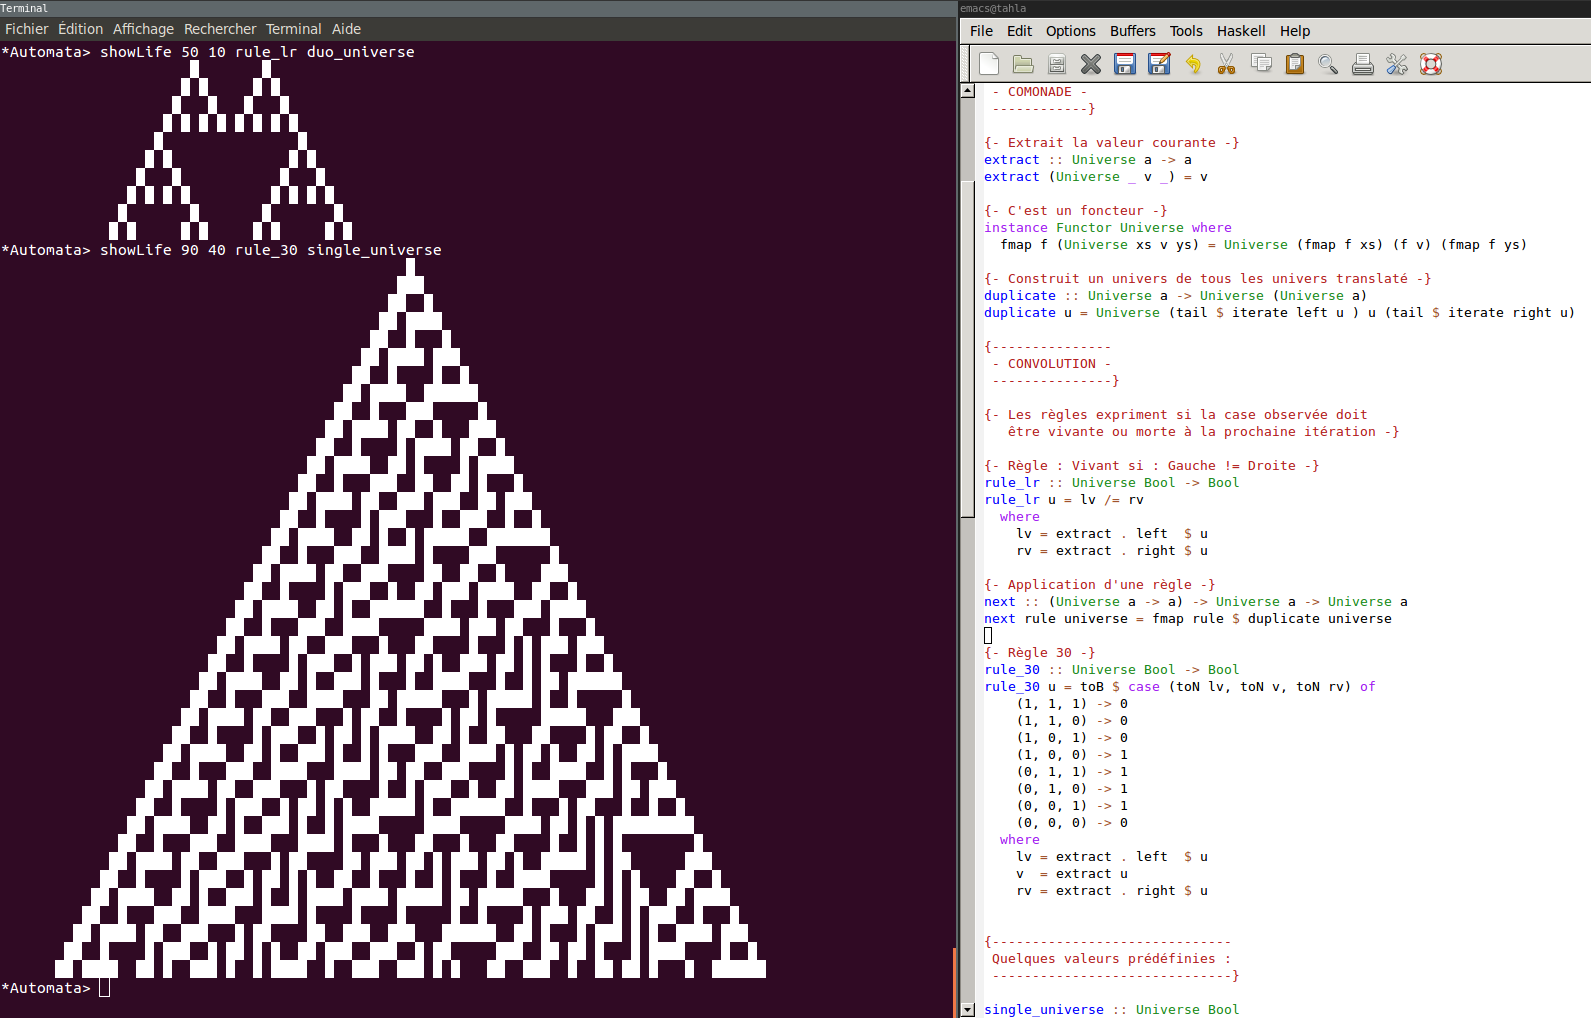
\includegraphics[scale=0.21]{live.png}
\end{center}
\end{frame}

\begin{frame}
\begin{center}

\includegraphics[scale=1]{chaton.png}
\end{center}
\begin{center}
Merci pour votre attention!
\end{center}

\end{frame}

\end{document}
